%!TEX root = thesis.tex

\chapter{Literature Review}

Software visualisation is building momentum within the space of live coding. This section seeks to identify the reason for this momentum and identify the purpose and potential for visualisations within this field.

% • Provide a context for the research 
% • Justify the research 
% • Ensure the research hasn't been done before (or that it is not just a "replication 
% study") 
% • Show where the research fits into the existing body of knowledge 
% • Enable the researcher to learn from previous theory on the subject 
% • Illustrate how the subject has been studied previously 
% • Highlight flaws in previous research 
% • Outline gaps in previous research 
% • Show that the work is adding to the understanding and knowledge of the field 
% • Help refine, refocus or even change the topic 

\section{Software}

Understanding changing software is one of the most important goals within the space of software engineering practice~\cite{Tao2012}. It is the nature of software to change~\cite{Purushothaman2005} and there is a need for not only the programmer to understand the software but also a knowledge transfer to take place between those creating the software and those observing the software as it changes~\citetemp{x}.

Programming languages are the formal languages of software. These languages are typically represented by source code in a plain text format. Plain text format is limited requiring an interpretation step (parsing and compilation) to acheive a functioning program~\cite{Badros2000}.

The concept of alternative source code representations is not new. Alternative representations of the source code have historically included diagrams~\citetemp{x} and, more recently, visual languages~\citetemp{x}. These vary greatly in the relation to the source code with some representations presenting a highly simplified source code representation compared to finer grained specific representatios~\citetemp{x}.

Although it is the nature of software to change, static diagrams have traditionally been used to represent software systems. These diagrams typically show the structure (class diagrams) or function (state diagrams) of a software system at a specific moment in time~\cite{Rumbaugh2004}. The usefulness of these diagrams lies in their ability to represent fundamental structures within the program more concisely than the source code itself~\citetemp{x}. However, the usefulness of these diagrams declines as they become more comprehensive and less abstract~\citetemp{x}. These diagrams must be continuously updated or generated to keep up with the ever changing software~\citetemp{x}.

Visual languages provide an alternative method of interaction with the software development process. However, visual languages are often not suited to general purpose programming~\cite{Myers1989}, providing only a subset of a full-featured text-based language.

The limitations of text-based languages have been identified...
-studies hint at the need for alternative representations of software and evaluation of their effectiveness.

There has not been extensive examination of the effectiveness of alternative representations of software...

The relationship between the source code and the running program must be defined...

\section{Visualisation}

Visualisation is widely understood as ``the use of computer-supported, interactive, visual representations of data to amplify cognition''~\cite{Card1999}. Further extensions of this definition discuss the need to transfer knowledge~\cite{Burkhard}. These definitions are summarised in the model shown in Figure~\ref{fig:model-of-visualisation}.

\begin{figure}
  \centering 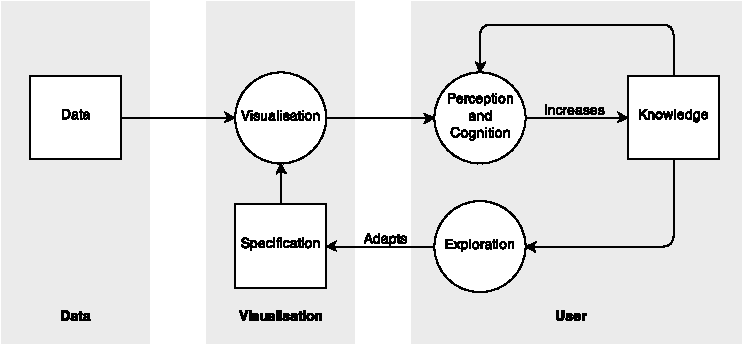
\includegraphics[width=\columnwidth]{../images/diagrams/wijk-model-of-visualisation.pdf}
  \caption{Generic model of visualisation \protect\cite{VanWijk2005}.}
\label{fig:model-of-visualisation}
\end{figure} 

% some foundational softvis references
Software visualisation is the process of representing the characteristics of computer programs visually~\cite{Stasko1992} in order to improve understanding~\cite{Diehl2007}. The advantage of providing a visual representation over the more traditional text-based representation is that the text-based approach does not take full advantage of the human visual information processing capability~\cite{Myers1989}.

Initial efforts to classify software visualisations identified two axes: whether the visualisation illustrated the code, the data or the algorithm and whether the visualisation was static or dynamic~\cite{Myers1989}. Following taxonomies characterised software visualisations according to the aspect of the program, the abstractness of the visualisation, the animation and the automation of the visualisation~\cite{Stasko1992}.

% From ozchi paper
Traditional approaches to software visualisation (see~\cite{Novais2013} for a review) often focus on structure of the source code (e.g. visualising complex object/class relationships) rather than the \emph{process} of programming. In a process-oriented activity such as live coding, different code visualisation techniques are necessary~\cite{McLean2010a,Magnusson2013}. However, these academic treatments of code visualisation in live coding adopt a survey-based approach, and the techniques discussed have not been subject to empirical evaluation.

Visualisations have the capacity to present information more effectively than traditional programming languages. Nevertheless, software visualisations still require significant development to benefit in the understanding of the complexity of software ~\cite{Baecker1995}. Effective software visualisations contribute to making software easier to understand, reflecting the software's history through the lifecycle, facilitating the transfer of knowledge from the programmer to the observer, making important structures visible and managing software complexity~\cite{Baecker1995}.

% \section{Visual Mapping (notes)}

% % Old stuff - temp
% The Early History of Software Visualization (Baecker, Ronald chapter of book) discusses the purpose of software visualisation as enhancing program representation, presentation and appearance. Discusses further that programmers have always used visualisation tools (eg. diagrams) to aid in illustrating program function, structure and process. States further that any of typography, symbols, images, diagrams and animation can present information more concisely than formal/natural programming languages.

% % Old stuff - temp
% The major `threads' of activity in the development of software visualsation as (1) the presentation of source code, (2) representation of data structures, (3) animation of program behaviour and (4) systems for software visualisation and (5) animation of concurrency~\cite{Baecker1995}.

% % Old stuff - temp
% Information visualisations can be constructed by mapping one data dimension to brightness, colors or orientations, however, it goes on to say that in practice this does not work very well. In particular, ``humans can only perceive a limited number of data dimensions''~\cite{Green}.

% % Old stuff - temp
% Discusses fundamental graphic primitives/procedures as invariants, components, correspondences and marks. Components define variational concepts. Invariants relate components. Marks (three types/``implantations'' including point, line and area) are graphical representations on the visualisation that represent invariants. Correspondences are the relationships between and among components.

% % Old stuff - temp
% There are two ``functionally different classes of visual variable''~\citetemp{x} including planar and retinal variables. Planar includes any spatial information and retinal variables include things such as size, color, shape, orientation, texture and brightness (which can use marks to be displayed).

% % Old stuff - temp
% Traditional software visualisation falls into a variety of categories. Each visualisation category corresponds to a reason for visualising the code.\\
% -what are the categories?\\
% -what reason for visualising the code do the categories correspond to?

% % Old stuff - temp
% The (abstract/graphical/animated) approach provides the basis for effective visualisations. Effective visulisations...\\
% -what do effective visualisations do?\\
% -what do effective visualisations achieve?

\section{Live Coding}

Live coding can be broadly defined as writing a program while it runs~\cite{Ward2004}. More specifically, live coding is identified as the artistic process of musical and visual expression through programming~\cite{Collins2003}.

% Why live code?\\
% -what does liveness mean? \cite{Auslander}\\
% -what does it contribute?\\
% -relation to improvisation?\\
% -computational creativity. \cite{Mclean}

Live coding is in a unique position to combine both source code and software visualisation techniques~\cite{McLean2010a}. This is due to the approach of live coding involving effective sensory communication, a goal of transparency of the coding process, and direct manipulation and refinement of the running program. These approaches are outlined below.

Live coding is built around communicating visually and audibly. This extends beyond the physical process of programming. Human input is visible in the creative process, demonstrating a link between physical actions and artistic output \cite{Mclean}.

Live coding has a history exposing audiences to code with the goal of live coding to ensure the transparency of the coding process~\cite{Collins2011,McLean2010a}. It provides a space in which there is a direct mapping from the human interaction with the source code to the musical or visual output~\cite{Mclean}. This relationship allows for visuals to map the interaction with the output~\citetemp{x}.

Lastly, live coding allows for direct manipulation and refinement of the running program~\cite{Swift2013}. This provides the capacity for uninterrupted visualisation of the dynamic aspects of the program~\citetemp{x} combined with the static nature of the source code. Similarly, manipulation and refinement of the running program allows for manipulation of the software visualisation to effectively communicate intent~\citetemp{x}.

% Live coding can retain audience attention.\\
% -how does live coding maintain attention?\\
% -can retain attention through the output (music), the process (programming) or the field (technology).

% % Old stuff - temp
% Live coding is a good application space for visualisations. Visualisations are the natural progression of the medium following musical performance and there is yet to be significant contribution to the field.

% % Old stuff - temp
% Live coding is a good case study for visualisations. The live coding style of performance provides the basis for evaluation of the effectiveness of visualisation techniques.\\
% -why is it a good case study?\\
% -why is it good for visualisations?

\section{Enjoyment and Understanding}

There is currently a search for software visualisations that increase enjoyment and understanding~\cite{McLean2010a}. Here enjoyment refers to the perceived benefit gained from observing the visualisations regardless of the level of understanding. Understanding refers to the ability of an observer or audience to comprehend the abstract thinking process of the programmer.

Enjoyment is the most common reaction to the positive effect of media~\cite{Vorderer2004}. Increased enjoyment is one of the fundamental goals of the modern media entertainment industry and is usually characterised by ``pleasurable affective response to a stimulus''~\cite{Brock2004}. 

Enjoyment results in increased attention to the stimulus and has been suggested to increase learning outcomes~\citetemp{x}.\\
-how do these factors relate to understanding?\\
-how do these factors relate to visualistions?\\
-how can these two factors contribute to effective visualisations?\\
-the concept assignment problem. \cite{Biggerstaff1994} (this paper may also be useful for explaining what understanding is in the context of software)

Understanding of a particular program is said to be achieved when the program can be explained ``in terms that are qualitatively different from the tokens used to construct the source code''~\cite{Biggerstaff1994}. Source code comprehension has a large body of research both within the understanding of text-based source code~\citetemp{x} and within the space of software visualisation~\cite{Hosking2005}.

In the space of live coding, this understanding is required to avoid a sense of distraction or exclusion~\cite{McLean2010a}. Furthermore, understanding software while it is changing presents an additional challenge~\cite{Eisenbarth2003}.

Understanding and enjoyment are often considered opposite concepts when implementing strategies to increase one or the other. 
-enjoyment is not completely separable from understanding. (not dual?)\\
-why can we not separate the two?\\
-what is the duality?\\
-how does this relate to visualisations?

\section{Didacticism and Aestheticism}

Enjoyment and understanding are often closely associate with the concepts of didacticism and aestheticism.

Didacticism refers to the ultimate goal of teaching. This approach mirrors the concept of understanding from the previous section. A didactic approach intends to increase the level of understanding.\\
-what is didacticism?\\
-how does it relate to visualisations?\\
-how does it relate to education?

On the other hand, aestheticism refers to the ultimate goal of appealing to the senses. This approach mirrors the concept of enjoyment from the previous section. An aesthetic approach intends to increase visualisation usability and increase retention~\cite{Cawthon2007}. Live coding has much potential and opportunity to evaluate and improve aesthetic effect~\cite{Bell}.

The artistic nature of the live coding field cannot be ignored when evaluating the effect of aesthetic and didactic approaches on the enjoyment and understanding of the audience.\\
-how does it relate to art?\\
-why is it still a good approach for evaluating understanding.

Software visualisations within the space of live coding have the potential to manipulate these two variables. For example, by increasing visual interest it may be possible to increase aesthetic appeal while reducing didacticism due to increased complexity and confusion~\citetemp{x}.

Questions raised within the literature suggest that it may be possible to combine or balance the goals of didacticism and aestheticism in order to manipulate understanding and enjoyment~\citetemp{x}. On the other hand, it may be that these two concepts cannot be completely separated. This will be further examined in the following sections.

The educational aspects of software visualsations have been examined in some studies~\citetemp{x,x} though few have applied these visualisations to areas outside of the commercial software development areas.

There has been an initial examination of the aesthetics in graph drawing~\citetemp{x} and within the space of software graph visualsations~\citetemp{x}, though no studies have examined the effectiveness of process-driven software visualisations. This is particularly the case for the examination of live coded visualisations and the effect on audiences.

Some frameworks for both aesthetic evaluation of visualisations
~\citetemp{x} and didactic evaluation of visualisations~\citetemp{x} have been developed though a thorough evaluation of the combination of the two concepts has not been considered~\citetemp{x}.

% Final words
Reviewing the model in Figure~\ref{fig:model-of-visualisation} from the didactic and aesthetic perspective identifies one major limitation. Within this model, a gain in knowledge is the only measurement of value.
-the literature has identified a need to redefine the model in terms of the relationship between understanding and enjoyment, didacticism and aestheticism.


